\subsection{Einleitung}
    Eine physikalische Groesse ist eine quantitativ bestimmbare Eigenschaft von Materie (die Masse eines Steins). Ein Groessenwert ist ein Produkt aus einem Zahlenwert und einer Masseinheit (der Stein wiegt 30kg). 
    \newline
    Eine Groessengleichung ist eine Beziehung zwischen physikalischen Groessen (die Flaeche des Steins setzt sich aus der Breite und der Laenge zusammen).
    \newline
    Das Problem bei Groessengleichung sind oft die unterschiedlichen Zehnerpotenzen. Dafuer gibt es einfache Regeln.
    \subsubsection{Potenzregeln}
        $x^{a} \times x^b = x^{a + b} \iff 10^2 \times 10^3 = 10^{2 + 3} = 10^5$
        \newline
        $\frac{x^a}{x^b} = x^{a - b} \iff \frac{10^4}{10^2} = 10^{4 - 2} = 10^2$
        \newline
        $(x^a)^{^{b}} = x^{a \times b} \iff (10^2)^{^{3}} = 10^{2 \times 3} = 10^6$
        \newline
        $a^n \times b^n = (a \times b)^n \iff 2^2 \times 3^2 = (2 \times 3)^2 = 6^2$
        \newline
        $\frac{a^n}{b^n} = (\frac{a}{b})^n \iff \frac{8^2}{4^2} = (\frac{8}{4})^2 = 2^2$
        \newline

    \subsubsection{SI-Einheiten}
        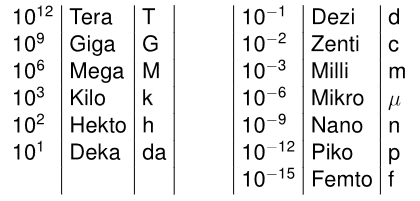
\includegraphics[]{Bilder/MINT/SI.png}
    \newpage
    
\newpage